
\documentclass[11pt]{article}
\addtolength{\oddsidemargin}{-1.cm}
\addtolength{\textwidth}{2cm}
\addtolength{\topmargin}{-2cm}
\addtolength{\textheight}{3.5cm}
\newcommand\tab[1][1cm]{\hspace*{#1}}
\usepackage[pdftex]{graphicx}
\usepackage{pdflscape}
\usepackage[T1]{fontenc}
\usepackage{hyperref}
\usepackage{float}
\usepackage{cite}
\hypersetup{
	colorlinks=true,
	linkcolor=black,
	filecolor=magenta,
	urlcolor=cyan,
}

% define the title
\author{Binary Ninjaz}
\title{EPI-USE -- NFC Business Cards}
\begin{document}
\begin{titlepage}
	
	\begin{center}
		% Upper part of the page         
       
		\textsc{\LARGE Binary Ninjaz}\\[0.3cm]
		% Title
		\rule{\linewidth}{0.5mm} \\[1cm]
		{ \huge \bfseries EPI-USE - NFC Business Cards}\\[0.5cm]
		\rule{\linewidth}{0.5mm} \\[1cm] 		
  
		
		\begin{minipage}{0.4\textwidth}
			\begin{flushleft} \large
				\emph{} \\
				Sizo {Duma}
			\end{flushleft}
		\end{minipage}
		\begin{minipage}{0.4\textwidth}
			\begin{flushright} \large
				\emph{} \\
				15245579
			\end{flushright}
		\end{minipage}

		\begin{minipage}{0.4\textwidth}
			\begin{flushleft} \large
            	\emph{} \\
				John {Ojo}
			\end{flushleft}
		\end{minipage}
		\begin{minipage}{0.4\textwidth}
			\begin{flushright} \large
				\emph{} \\
				15096794 
			\end{flushright}
		\end{minipage}
		
		\begin{minipage}{0.4\textwidth}
			\begin{flushleft} \large
				\emph{} \\
				Kevin Reid
			\end{flushleft}
		\end{minipage}
		\begin{minipage}{0.4\textwidth}
			\begin{flushright} \large
				\emph{} \\
				15008739
			\end{flushright}
		\end{minipage}

		\begin{minipage}{0.4\textwidth}
			\begin{flushleft} \large
				\emph{} \\
				Shaun {Yates}
			\end{flushleft}
		\end{minipage}
		\begin{minipage}{0.4\textwidth}
			\begin{flushright} \large
				\emph{} \\
				16007493
			\end{flushright}
		\end{minipage}
        
        \begin{minipage}{0.4\textwidth}
			\begin{flushleft} \large
				\emph{} \\
				Letanyan {Arumugam}
			\end{flushleft}
		\end{minipage}
		\begin{minipage}{0.4\textwidth}
			\begin{flushright} \large
				\emph{} \\
				14228123 
			\end{flushright}
		\end{minipage}
		
		\begin{minipage}{0.4\textwidth}
			\begin{flushleft} \large
				\emph{} \\
				Teboho {Mokoena}
			\end{flushleft}
		\end{minipage}
		\begin{minipage}{0.4\textwidth}
			\begin{flushright} \large
				\emph{} \\
				14415888 
			\end{flushright}
		\end{minipage}
		\break
		\break
		
		\rule{\linewidth}{0.5mm} \\[1cm] 
	
		\newline
		\begin{minipage}{0.9\textwidth}
			\begin{center} \large
				\emph{} \\
            \includegraphics[width=1\linewidth]{TeamPic.JPG}
            \end{center}
        \end{minipage}
    % 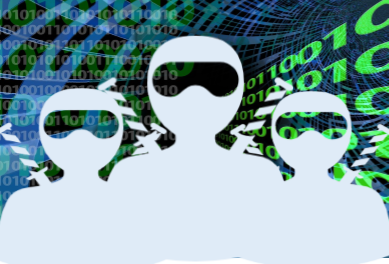
\includegraphics[width=0.7\linewidth]{Images/binaryNinjaz.PNG}\\[1cm] 
			\textsc{\Large Stakeholders}\\[0.8cm]	
		
		\begin{minipage}{0.5\textwidth}
			\begin{flushleft} \large
				\emph{} \\
				EPI-USE Africa
			\end{flushleft}
		\end{minipage}
		\begin{minipage}{0.4\textwidth}
			\begin{flushright} \large
				\emph{} \\
				Mvuyisi Scheepers
			\end{flushright}
			\newline
		\end{minipage}
	\end{center}
\end{titlepage}
\tableofcontents


\section{Binary Ninjaz}
\subsection{About Us}
Binary Ninjaz is a diverse team of young, hard working and passionate software developers. Each member of the team brings their own unique diverse skill set to the table. These include competence in a wide range of fields such as: Artificial Intelligence, Multimedia, Mathematics and also Business. Binary Ninjaz has a fun and modern culture that promotes "blue sky thinking" and solutions that fit into the modern environment. The team works exceptionally well together and all members aim to produce a quality product while also creating a constructive relationship with our client.


\subsection{The Team}




\subsubsection{Sizo Duma} 
\paragraph{}Course : BSc Information Technology (Software Development stream)
\paragraph{} Career Interest : Software & Systems Engineering, Moblie Application Developer 
\paragraph{}Skills : 
\begin{itemize}
\item Programming (C, C++, Java, C\#, XML, JavaScript, PHP, HTML5, CSS3)
\item Advanced Database Systems (Relational, Document \& Object Oriented)
\item Systems Modelling/Design
\item Mobile Development (Android Studio)
\item Web Development (LAMP \& WAMP)
\end{itemize}
\paragraph{Bio :}I started at the University of Pretoria in studying BSc Computer Science. The following decided to switch to the BSc Information Technology program which allowed me to take Computer Science along with Informatics as a second major. I did this because while I am highly passionate about the deeper back-end development that Computer Science targets. I also like business. I particularly like the business aspect of IT along with front-end development, and wish to attain as much knowledge as I can about: systems development, front-end development, and back-end development which are all catered for best in BSc Information Technology (Software Development). I am passionate about what I am studying which makes putting in the extra effort to always produce a perfect product that much easier. 

\subsubsection{John Ojo}
\paragraph{}Course : BSc Information Technology \& Applied Mathematics
\paragraph{}Career Interest : Software Developments/Engineering, Financial/System Analyst
\paragraph{}Skills : 
\begin{itemize}
\item Programming (C++, Java, MATLAB, SAS, Assembly)
\item Web development
\item Database Systems (Relational)
\end{itemize}
\paragraph{Bio :} Since the beginning of my degree I have been looking forward to doing 
Software Engineering. I wanted to combine different systems, mix the old 
and the new and especially combine mathematics and Information 
Technology. Mathematics has been the one subject that has been getting 
the best of students since the beginning and IT is the new world that 
everyone wants to be part of. I chose to do both to truly defeat something 
that has challenged to students and join the world of IT where concepts 
and theories were made possible. I want to work with different people, 
create things that were just thoughts and improve life as a whole. IT gives 
me that opportunity.

\subsubsection{Kevin Reid}
\paragraph{}Course : BSc Computer Science
\paragraph{}Career Interest : Software Development, Game Development
\paragraph{}Skills : 
\begin{itemize}
\item Programming: C, C++, Java, Assembly (x86), HTML, JavaScript, CSS, MySQL (MariaDB), PHP, XML, BASH, ZSH, LaTeX.
\item GNU/Linux (Debian and Arch based)
\item 3D modelling and texturing (Blender)
\item Circuitry and Electronics
\item LAMP Stack
\end{itemize}
\paragraph{Bio :} I came out of high school and went into computer engineering for a year and a half, after only enjoying the computer science modules, I decided it was time to make a change. Since that change, I have grown to love almost all things computer science, and have never been happier.
In my spare time I tend to enjoy video games, series and movies. But otherwise, I take great pleasure in programming--nothing better than a good challenge--or other computer related things; like when you have over 60 mods (it's not many I know) in Skyrim and it all works--then you realise that that's actually the best part of the game; or learning Dvorak was great fun; blender's my on and off again lover; installing and configuring an operating system is always a hoot--speaking of: it's time I installed Arch again. . .


\subsubsection{Shaun Yates}
\paragraph{}Course : BSc (Information Technology) – Information and Knowledge Systems
\paragraph{}Career Interest : Artificial Intelligence
\paragraph{}Skills :  
\begin{itemize}
\item Programming (C++, Java, MySQL, HTML, CSS, JavaScript, PHP)
\item Database Systems (Relational)
\item Systems Design/Modelling
\end{itemize}
\paragraph{Bio :} I was shown the world of IT at a young age due to my dad being an IT consultant, which helped show me that a career in IT is what I want 
to do with my life. I started my course in 2016, originally taking the Genetics elective group due to it interesting me; it also allowed 
me to take Artificial Intelligence in third year, which few elective groups allow. Now, in third year, I got the choice to take more 
Computer Science related modules instead of the Genetics electives, and I opted for that instead. In my spare time I enjoy series or 
going out and meeting new people. I like to think I’m a very sociable person and look forward to working with many different people in 
the years to come, as I firmly believe you can learn a lot from anybody that you meet.

\subsubsection{Letanyan Arumugam}
\paragraph{}Course : BSc Computer Science 
\paragraph{}Career Interest : Software Engineering
\paragraph{}Skills :
\begin{itemize}

\item Programming Language: C, C++, Java, Swift, Objective-C, SQL, Python, Delphi, x86 ASM, HTML, JavaScript, CSS, PHP, Bash.
\item macOS, iOS, tvOS, watchOS development
\item Windows development 
\item Web Development
\item Known Technologies: MAMP Stack, Git, XCode
\end{itemize}
\paragraph{Bio :}I am currently a 3rd-year student at the University of Pretoria studying BSc Computer Science. In my spare time, I'm an active member of the Swift-Evolution community, which deals with the language design of, the programming language, Swift. With Swift, I have created applications that have were published on the Apple App Store. Building these apps allows me to do a few things that I enjoy. These would be algorithm optimisation, user experience and designing an excellent looking user interface.

\subsubsection{Teboho Mokoena}
\paragraph{}Course : BSc Information Technology 
\paragraph{}Career Interest : Software Engineering, Systems Analyst
\paragraph{}Skills :
\begin{itemize}
\item Programming (and Netcentric) Languages: C++, Java, C, C sharp, MongoDB, NodeJS, Javascript, PHP
\item Android Application Development and .Net Application Development
\item Software Modelling, Operating System and Concurrent Systems
\item API and REST Architecture interfaces
\item Xamarin Mobile Application development
\end{itemize}
\paragraph{Bio :} Teboho Vincent Mokoena, born and raised in Qwa-Qwa, Free State. Enrolled in
the BSc It (Knowledge and Information system) programme at the University of
Pretoria, in the year 2015. Majoring in Computer Science (Software
Development elective group). Active member of World CodeSprint 12 coding
contest orginisation since 2016.

\section{Motivation For Project}
When deciding what projects to bid for because of the diverse personnel on our team, it was a bit tough picking one project we all agreed upon. We tackled this issue by having each team member make a top five list of projects which they were interested in. The NFC Business Cards was not only suggested by every member but ranked high on every members list, and at the same time was the only project we all had mutual interest in. This common interest has led to this being our first choice option by far and we believe that this also increases the chances of project success and us working well together on it to produce a top-level system as we are all willing to go the extra mile on this project.
\newline
\newline Every team member also has skills that will contribute to making this a successful project. The team has members who major in Computer Science, Informatics, Mathematics \& Multimedia. The Multimedia \& Informatics members will focus on the front-end development of the project and produce a system with a flawless user experience and interface. The Mathematics and some Computer Science team members will be more focused on the backend, data management part of the system and enforce things such as security and efficiency.
\newline
\newline We are the best choice for this project because of our diverse skills and excellent team work. With our common interest in this project we aim at doing our best to meet all the client's requirements and exceed expectations.

\section{The Project}
\subsection{High Level Description}
The project is to develop an efficient and effective system of electronic business cards making use of devices such as our Smartphones and possibly 3rd party electronic NFC cards. The System should make collection of potential client or giving out of business information more convenient through the use of one device rather than plenty of physical cards (which may sometimes get lost and are costly long term), and it should make it much more seamless with the use of NFC technology. It will automate features such as sending fist contact mail, and adding relevant contact info either your email address book or contact book if it's first contact. The system should also be able to extend to other social media platforms such as Linked In, Facebook and more.
\newline
\newline The following requirements will be met : 
\begin{itemize}
\item The ability to seamlessly transfer contact (business card) data  between two devices.
\item Automation of general tasks such as first contact mail between first time interactions.
\item A safe and secure platform for data gathering \& sharing.
\item and more feature to be determined.
\end{itemize}

\subsection{The Domain Model}
\includegraphics[width=1\linewidth]{DM.jpg}
           

\subsection{Technologies To Be Used}
\begin{itemize}
\item NFC Enabled Smart Mobile Phones
\item Android Studio For App Development
\item Java For Backend Development
\item Android SQLlite/MySQL
\item Google/Amazon Cloud Services
\item Other: 3rd party NFC enabled cards 
\end{itemize}
\subsection{Development Methodology}
\paragraph{} We will be utilising \textbf{Agile} development methodologies. We believe that this is the best means to enable both us as the engineering team and the client to focus on effectively performing the tasks integral to successfully providing the desired Business Card system for this project. EPI-USE will take the part as Product Owner and we as the Binary Ninjaz will assume the role of the Development Team. 

\paragraph{} 
Interactions are highly valued by our team, hence we are dedicated to conducting meetings fortnightly (or weekly should the need occur) with EPI-USE to ensure we are on course with the clients expectations.This will also serve and start and end points for Sprints (which serve as schedules for delivery of agreed upon requirements). We will also be regularly meeting and consulting with our lectures and tutors for further guidance throughout the duration of the project. All of the above mentioned parties will have access a third party instant messaging platform (Slack, WhatsApp) in order to facilitate communication apart from physical meetings which can be on a daily basis.

\paragraph{} 
We hope to employ a collaborative and cooperative approach between us and both stakeholders for the life span of the project. we will frequently be working on the project and providing incremental deliverables to the client. 

\paragraph{}
The role we expect EPI-USE to play is:
\newline You take an active involvement and collaboration in all phases of project, aid us with the Analysis and Design to ensure correct functionality, Periodically review the product in order to ensure  is in line with expectations, and to provide us with the means (NFC enabled cards) to produce an effective end product.

\begin{center}
{\fontfamily{UWR Grotesk}\sffamily\bfseries
\large Thank You EPI-USE Africa. The Binary Ninjaz look forward to working with you in the near future.
}
\end{center}

\end{document}
